\chapter{Implementasi dan Pengujian}
\label{chap:implementasipengujian}

Bab ini membahas tentang implementasi dan pengujian perangkat lunak berdasarkan rancangan yang sudah dibuat. Ada dua jenis pengujian yang dilakukan, yaitu pengujian fungsional, pengujian keakuratan, dan pengujian eksperimental. Bab ini juga membahas tentang lingkungan yang digunakan untuk pengujian perangkat lunak ini.

\section{Lingkungan untuk Pengujian}
\label{sec:lingkunganpengujian}

Pengujian perangkat lunak ini dilakukan di Lab Komputasi FTIS Unpar ruang 9018. Semua \textit{file} permainan yang dipakai dalam pengujian ini dapat dilihat di bab Lampiran. 

Ada dua jenis lingkungan untuk pengujian perangkat lunak ini, yaitu:

\begin{enumerate}
\item Lingkungan perangkat keras, yaitu lingkungandigunakan untuk pengujian perangkat lunak ini memiliki spesifikasi berikut:

\begin{table}
\centering
\captionsetup{justification=centering}
\caption[Lingkungan perangkat keras untuk pengujian perangkat lunak]{Lingkungan perangkat keras untuk pengujian perangkat lunak}
\begin{tabular}{| l | l |}
\hline
Parameter & Nilai \\
\hline \hline
\textit{Processor} & Lorem Ipsum \\
\hline
\textit{RAM (Random Access Memory)} & Lorem Ipsum \\
\hline
\textit{VGA (Video Graphics Array)} & Lorem Ipsum \\
\hline
\end{tabular}
\label{tab:lingkunganpk}
\end{table}

\item Lingkungan perangkat lunak, yaitu lingkungan yang digunakan untuk pengujian perangkat lunak ini memiliki spesifikasi berikut:

\begin{table}
\centering
\captionsetup{justification=centering}
\caption[Lingkungan perangkat lunak untuk pengujian perangkat lunak]{Lingkungan perangkat lunak untuk pengujian perangkat lunak}
\begin{tabular}{| l | l |}
\hline
Parameter & Nilai \\
\hline \hline
Sistem Operasi & Lorem Ipsum \\
\hline
Bahasa Pemrograman & Java \\
\hline
\textit{IDE (Integrated Development Environment)} & NetBeans IDE 8.2 \\
\hline
\textit{Library Java} & JDK (\textit{Java Development Kit}) 1.8 \\
\hline
\textit{JVM (Java Virtual Machine)} & Java Version 8 Update Lorem Ipsum \\
\hline
\end{tabular}
\label{tab:lingkunganpl}
\end{table}

\end{enumerate}

\section{Implementasi}
\label{sec:implementasi}

Hasil implementasi dari rancangan perangkat lunak yang sudah dibuat ini terdiri dari dua bagian, yaitu:

\begin{enumerate}
\item Kode program
\item Antarmuka perangkat lunak
\end{enumerate}

Kedua bagian tersebut akan dijelaskan lebih lanjut di bawah ini.

\subsection{Kode Program}
\label{sec:kodeprogram}

Kode program untuk perangkat lunak ini ditulis dalam bahasa pemrograman Java, berdasarkan dengan rancangan diagram kelas yang sudah dibuat, seperti dapat dilihat pada sub-bab~\ref{sec:diagramkelas}. Seluruh kode program untuk perangkat lunak ini dapat dilihat di bab Lampiran.

\subsection{Antarmuka Perangkat Lunak}
\label{sec:antarmukapl}

Antarmuka untuk perangkat lunak ini dirancang berdasarkan rancangan yang sudah dibuat, seperti dapat dilihat pada sub-bab~\ref{sec:perancanganantarmuka}.

Gambar~\ref{fig:antarmukapl1} menunjukkan antarmuka perangkat lunak saat pertama kali dibuka, sebelum \textit{file} permainan dibuka. Gambar~\ref{fig:antarmukapl2} menunjukkan kotak dialog untuk memilih \textit{file} permainan yang akan dibuka. Gambar~\ref{fig:antarmukapl3} menunjukkan antarmuka perangkat lunak setelah membuka \textit{file} permainan yang dipilih. Gambar~\ref{fig:antarmukapl4} menunjukkan kotak dialog untuk mengatur nilai untuk parameter-parameter algoritma genetik. Gambar~\ref{fig:antarmukapl5} menunjukkan antarmuka perangkat lunak setelah permainan berdasarkan \textit{file} permainan yang telah dibuka diselesaikan.

\begin{figure}
\centering
\captionsetup{justification=centering}
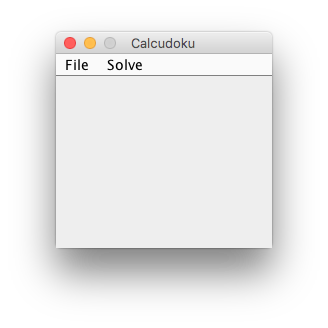
\includegraphics[scale=0.5]{Gambar/ImplementasiPengujian/Calcudoku1.png}
\caption[Antarmuka perangkat lunak saat pertama kali dibuka]{Antarmuka perangkat lunak saat pertama kali dibuka}
\label{fig:antarmukapl1}
\end{figure}

\begin{figure}
\centering
\captionsetup{justification=centering}
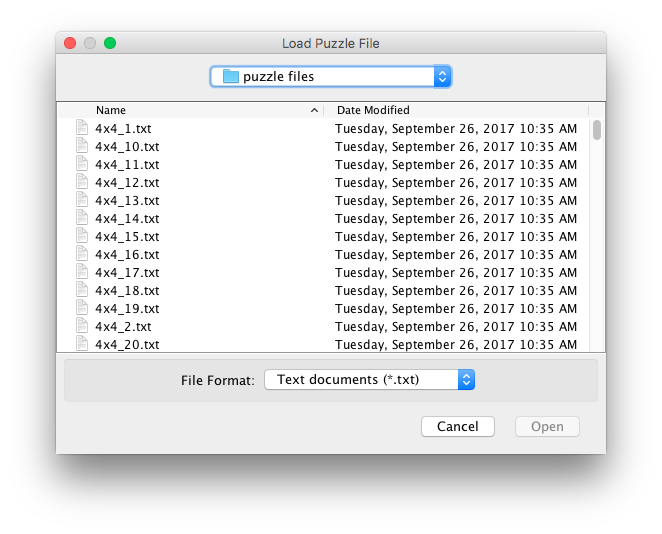
\includegraphics[scale=0.5]{Gambar/ImplementasiPengujian/FileChooser.png}
\caption[Kotak dialog untuk memilih \textit{file} permainan yang akan dibuka]{Kotak dialog untuk memilih \textit{file} permainan yang akan dibuka}
\label{fig:antarmukapl2}
\end{figure}

\begin{figure}
\centering
\captionsetup{justification=centering}
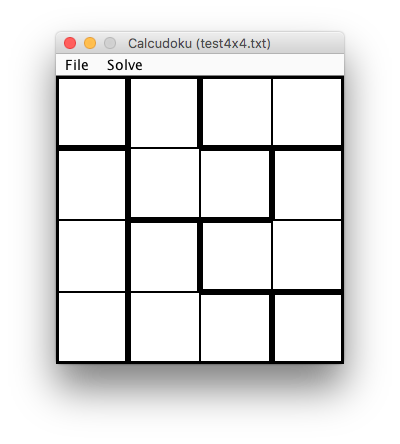
\includegraphics[scale=0.5]{Gambar/ImplementasiPengujian/Calcudoku2.png}
\caption[Antarmuka perangkat lunak sesudah membuka \textit{file} permainan yang dipilih]{Antarmuka perangkat lunak sesudah membuka \textit{file} permainan yang dipilih}
\label{fig:antarmukapl3}
\end{figure}

\begin{figure}
\centering
\captionsetup{justification=centering}
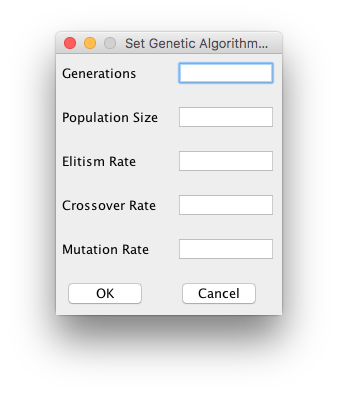
\includegraphics[scale=0.5]{Gambar/ImplementasiPengujian/SetGAParameters.png}
\caption[Kotak dialog untuk mengatur nilai dari parameter-parameter algoritma genetik]{Kotak dialog untuk mengatur nilai dari parameter-parameter algoritma genetik}
\label{fig:antarmukapl4}
\end{figure}

\begin{figure}
\centering
\captionsetup{justification=centering}
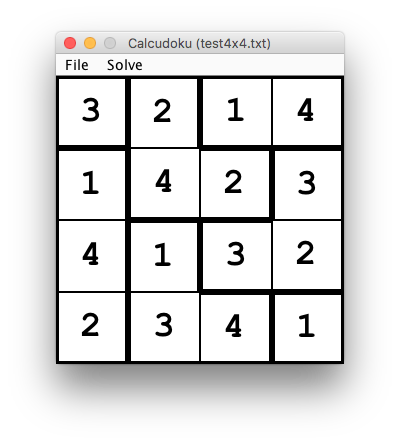
\includegraphics[scale=0.5]{Gambar/ImplementasiPengujian/Calcudoku3.png}
\caption[Antarmuka perangkat lunak setelah permainan berdasarkan \textit{file} permainan yang telah dibuka diselesaikan]{Antarmuka perangkat lunak setelah permainan berdasarkan \textit{file} permainan yang telah dibuka diselesaikan}
\label{fig:antarmukapl5}
\end{figure}

\clearpage

\section{Pengujian Fungsional}
\label{sec:pengujianfungsional}

Pengujian fungsional bertujuan untuk memastikan bahwa perangkat lunak dapat berfungsi sebagaimana mestinya. Skenario-skenario yang dilakukan dalam pengujian fungsional untuk perangkat lunak ini adalah:

\begin{enumerate}
\item Memilih menu \textit{item} "\textit{Reset Puzzle}", "\textit{Close Puzzle File}", dan "\textit{Check Puzzle}" dari menu "\textit{File}" atau menu \textit{item} "\textit{Backtracking}", "\textit{Hybrid Genetic}", dan "\textit{Set Genetic Algorithm Parameters}" dari menu "\textit{Solve}" sebelum membuka \textit{file} permainan.

Jika salah satu dari menu \textit{item} tersebut dipilih sebelum membuka \textit{file} permainan, maka pesan error "\textit{Puzzle file not loaded}" akan muncul, seperti dapat dilihat pada Gambar~\ref{fig:puzzlefilenotloaded}.

\begin{figure}
\centering
\captionsetup{justification=centering}
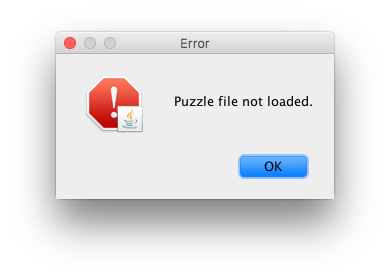
\includegraphics[scale=0.5]{Gambar/ImplementasiPengujian/PuzzleFileNotLoaded.png}
\caption[Kotak pesan error "\textit{Puzzle file not loaded}"]{Kotak pesan error "\textit{Puzzle file not loaded}"}
\label{fig:puzzlefilenotloaded}
\end{figure}

\item Memilih menu \textit{item} "\textit{Load Puzzle File}".

Jika menu tersebut dipilih maka akan keluar kotak pemilihan \textit{file} permainan, seperti dapat dilihat pada Gambar~\ref{fig:filechooser}. Pilihlah sebuah \textit{file} permainan yang ingin dibuka. Tekan tombol "OK" untuk membuka \textit{file} permainan tersebut, atau tekan tombol "\textit{Cancel}" untuk membatalkan proses membuka \textit{file} permainan.

\begin{figure}
\centering
\captionsetup{justification=centering}
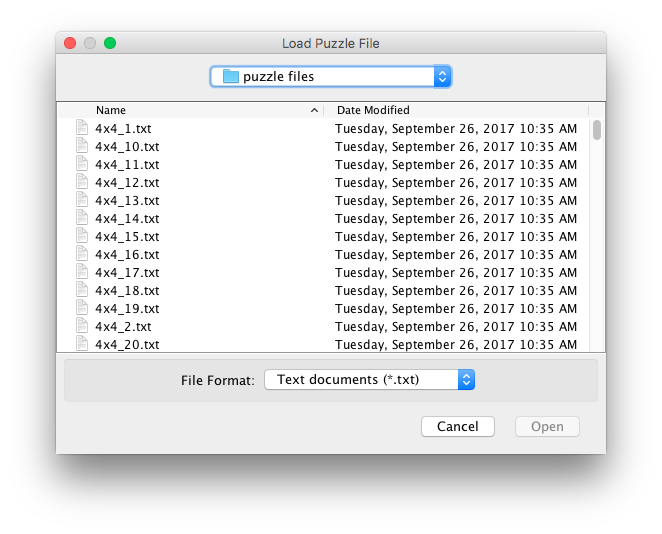
\includegraphics[scale=0.5]{Gambar/ImplementasiPengujian/FileChooser.png}
\caption[Kotak pemilihan \textit{file} permainan]{Kotak pemilihan \textit{file} permainan}
\label{fig:filechooser}
\end{figure}

Jika perangkat lunak sudah membuka sebuah \textit{file} permainan, maka akan keluar kotak dialog "\textit{Are you sure you want to load another puzzle file?}", seperti dapat dilihat pada Gambar~\ref{fig:loadpuzzlefile}. Tekan tombol "Yes" untuk membuka \textit{file} permainan tersebut, atau tekan tombol \textit{"No"} untuk membatalkan proses membuka \textit{file} permainan.

\begin{figure}
\centering
\captionsetup{justification=centering}
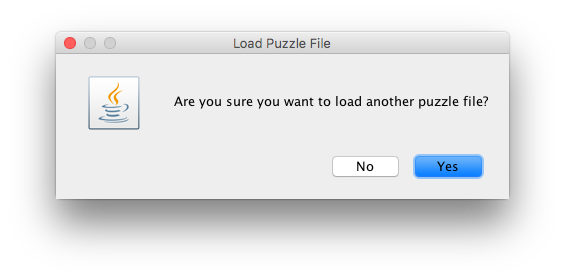
\includegraphics[scale=0.5]{Gambar/ImplementasiPengujian/LoadPuzzleFile.png}
\caption[Kotak dialog "\textit{Are you sure you want to load another puzzle file?}"]{Kotak dialog "\textit{Are you sure you want to load another puzzle file?}"}
\label{fig:loadpuzzlefile}
\end{figure}

Jika \textit{file} permainan yang dipilih berhasil dibuka, maka perangkat lunak akan menampilkan permainan berdasarkan \textit{file} yang dipilih, seperti dapat dilihat pada Gambar~\ref{fig:antarmukapl3}.

\textit{File} permainan untuk perangkat lunak ini adalah \textit{file} teks (*.txt). Format \textit{file} permainan yang valid dapat dilihat di sub-bab~\ref{sec:perancanganmasukan}.

Jika \textit{file} permainan yang dibuka tidak \textit{valid}, misalnya karena \textit{file} permainan yang dibuka bukan \textit{file} teks, atau jika \textit{file} teks yang akan dibuka formatnya tidak \textit{valid}, maka pesan error "\textit{Invalid puzzle file}" akan muncul, seperti dapat dilihat pada Gambar~\ref{fig:invalidpuzzlefile}.

\begin{figure}
\centering
\captionsetup{justification=centering}
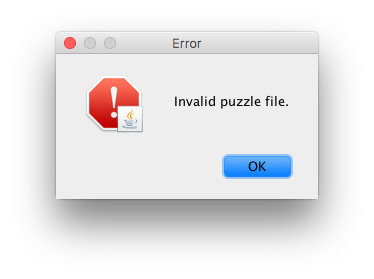
\includegraphics[scale=0.5]{Gambar/ImplementasiPengujian/InvalidPuzzleFile.png}
\caption[Pesan error "\textit{Invalid puzzle file}"]{Pesan error "\textit{Invalid puzzle file}"}
\label{fig:invalidpuzzlefile}
\end{figure}

Jika ada kesalahan dalam penentuan operator untuk \textit{cage} yang ada di dalam \textit{grid}, misalnya operator \begin{math}-\end{math}, atau \begin{math}\div\end{math} untuk \textit{cage} yang tidak berukuran 2 sel, operator \begin{math}+\end{math}, atau \begin{math}\times\end{math}, untuk \textit{cage} yang berukuran 1 sel, atau operator \begin{math}=\end{math} untuk \textit{cage} yang berukuran lebih besar dari 1 sel, maka pesan error "\textit{Invalid cages}" akan muncul, seperti dapat dilihat pada Gambar~\ref{fig:invalidcages}.

\begin{figure}
\centering
\captionsetup{justification=centering}
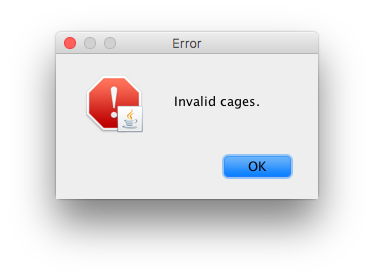
\includegraphics[scale=0.5]{Gambar/ImplementasiPengujian/InvalidCages.png}
\caption[Pesan error "\textit{Invalid cages}"]{Pesan error "\textit{Invalid cages}"}
\label{fig:invalidcages}
\end{figure}

Jika salah satu dari kedua error tersebut terjadi, maka akan keluar pesan error "\textit{Error in loading puzzle file}", seperti dapat dilihat pada Gambar~\ref{fig:errorinloadingpuzzlefile}.

\begin{figure}
\centering
\captionsetup{justification=centering}
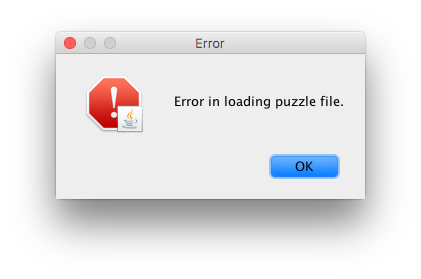
\includegraphics[scale=0.5]{Gambar/ImplementasiPengujian/Error.png}
\caption[Pesan error "\textit{Error in loading puzzle file}"]{Pesan error "\textit{Error in loading puzzle file}"}
\label{fig:errorinloadingpuzzlefile}
\end{figure}

\clearpage

\item Menyelesaikan permainan dengan usahanya sendiri

Jika pemain berhasil menyelesaikan permainan dengan usahanya sendiri, maka kotak informasi "\textit{Congratulations, you have successfully solved the puzzle}" akan muncul, seperti dapat dilihat pada Gambar~\ref{fig:congratulations}.

\begin{figure}
\centering
\captionsetup{justification=centering}
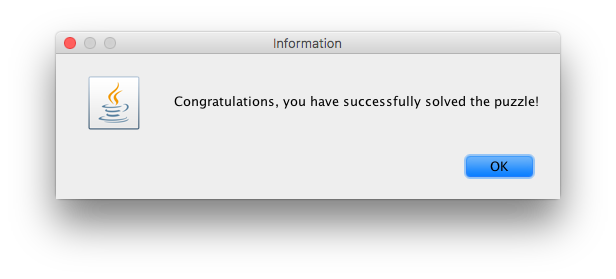
\includegraphics[scale=0.5]{Gambar/ImplementasiPengujian/Congratulations.png}
\caption[Pesan informasi "\textit{Congratulations, you have succesfully solved the puzzle}"]{Pesan informasi "\textit{Congratulations, you have succesfully solved the puzzle}"}
\label{fig:congratulations}
\end{figure}

\item Me-\textit{reset} permainan

Pemain me-\textit{reset} permainan dengan memilih menu \textit{item} "\textit{Reset Puzzle}" dalam menu "\textit{File}". Jika menu \textit{item} ini dipilih, maka akan keluar kotak dialog "\textit{Are you sure you want to reset this puzzle?}, seperti dapat dilihat pada Gambar~\ref{fig:resetpuzzle}. Tekan tombol "\textit{Yes}" untuk me-\textit{reset} permainan, atau tekan tombol "\textit{No}" untuk membatalkan proses \textit{reset} permainan.

\begin{figure}
\centering
\captionsetup{justification=centering}
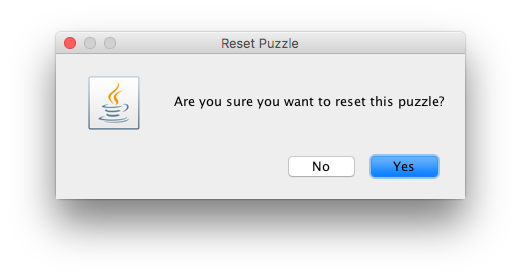
\includegraphics[scale=0.5]{Gambar/ImplementasiPengujian/ResetPuzzle.png}
\caption[Kotak dialog "\textit{Are you sure you want to reset this puzzle?}"]{Kotak dialog "\textit{Are you sure you want to reset this puzzle?}"}
\label{fig:resetpuzzle}
\end{figure}

\item Memeriksa permainan jika ada nilai yang salah di dalam \textit{grid}.

Perangkat lunak ini dapat memeriksa jika ada nilai yang salah di dalam \textit{grid} secara otomatis.

Jika ada nilai yang berulang dalam sebuah baris, maka akan keluar kotak informasi "\textit{Row} (nomor baris) \textit{has duplicate numbers}", seperti dapat dilihat pada Gambar~\ref{fig:rowduplicate}.

\begin{figure}
\centering
\captionsetup{justification=centering}
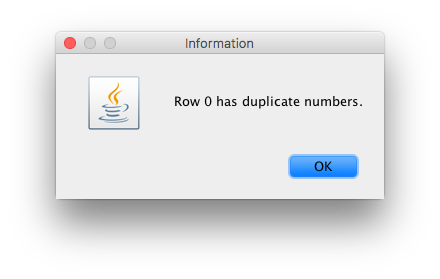
\includegraphics[scale=0.5]{Gambar/ImplementasiPengujian/RowDuplicate.png}
\caption[Pesan informasi "\textit{Row} (nomor baris) {has duplicate numbers}"]{Pesan informasi "\textit{Row} (nomor baris) \textit{has duplicate numbers}"}
\label{fig:rowduplicate}
\end{figure}

Jika ada nilai yang berulang dalam sebuah kolom, maka akan keluar kotak informasi "\textit{Column} (nomor kolom) \textit{has duplicate numbers}", seperti dapat dilihat pada Gambar~\ref{fig:columnduplicate}.

\begin{figure}
\centering
\captionsetup{justification=centering}
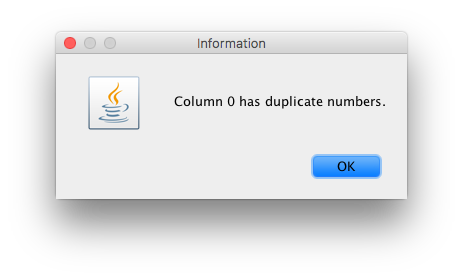
\includegraphics[scale=0.5]{Gambar/ImplementasiPengujian/ColumnDuplicate.png}
\caption[Pesan informasi "\textit{Column} (nomor kolom) {has duplicate numbers}"]{Pesan informasi "\textit{Column} (nomor kolom) \textit{has duplicate numbers}"}
\label{fig:columnduplicate}
\end{figure}

Jika nilai-nilai dalam sebuah \textit{cage} tidak mencapai nilai tujuan yang telah ditentukan jika dihitung dengan operasi matematika yang telah ditentukan, maka akan keluar kotak informasi "\textit{Values of cells in the cage do not reach the target number}", seperti dapat dilihat pada Gambar~\ref{fig:cagedonotreachtargetnumber}.

\begin{figure}
\centering
\captionsetup{justification=centering}
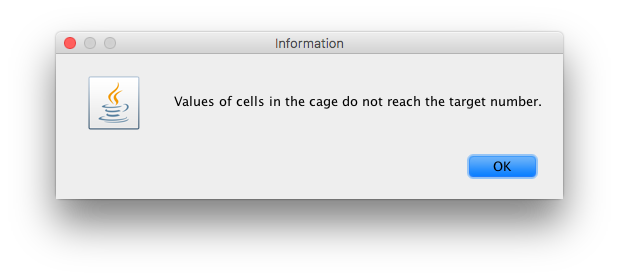
\includegraphics[scale=0.5]{Gambar/ImplementasiPengujian/CageDoNotReachTargetNumber.png}
\caption[Pesan informasi "\textit{Values of cells in the cage do not reach the target number}"]{Pesan informasi "\textit{Values of cells in the cage do not reach the target number}"}
\label{fig:cagedonotreachtargetnumber}
\end{figure}

Tetapi, pemain juga dapat meminta perangkat lunak untuk memeriksa permainan jika ada nilai yang salah di dalam \textit{grid} secara manual, dengan memilih menu \textit{item} "\textit{Check Puzzle}" dalam menu "\textit{File}".

Jika menu \textit{item} ini dijalankan, dan ternyata ada nilai yang salah di dalam \textit{grid}, maka akan muncul kotak informasi "\textit{There are cells with incorrect values in the grid}", seperti dapat dilihat pada Gambar~\ref{fig:incorrectvalues}.

\begin{figure}
\centering
\captionsetup{justification=centering}
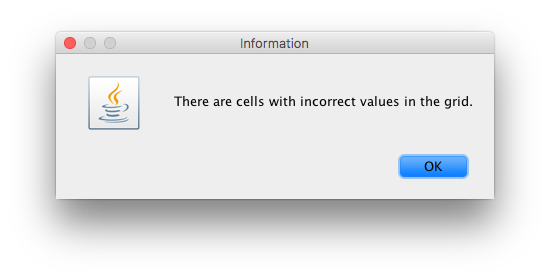
\includegraphics[scale=0.5]{Gambar/ImplementasiPengujian/IncorrectValues.png}
\caption[Pesan informasi "\textit{There are cells with incorrect values in the grid}"]{Pesan informasi "\textit{There are cells with incorrect values in the grid}"}
\label{fig:incorrectvalues}
\end{figure}

Jika menu \textit{item} ini dijalankan dan ternyata ada sel yang masih kosong, maka akan muncul kotak informasi "\textit{There are empty cells in the grid}", seperti dapat dilihat pada Gambar~\ref{fig:emptycells}.

\begin{figure}
\centering
\captionsetup{justification=centering}
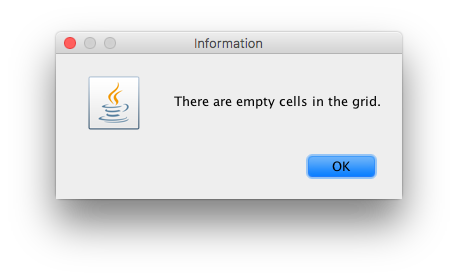
\includegraphics[scale=0.5]{Gambar/ImplementasiPengujian/EmptyCells.png}
\caption[Pesan informasi "\textit{There are empty cells in the grid}"]{Pesan informasi "\textit{There are empty cells in the grid}"}
\label{fig:emptycells}
\end{figure}

\item Mengatur nilai untuk parameter-parameter algoritma genetik

\end{enumerate}

\section{Pengujian Keakuratan}
\label{sec:pengujiankeakuratan}

Pengujian keakuratan dilakukan untuk memastikan bahwa permainan yang ditampilkan oleh perangkat lunak sesuai dengan \textit{file} permainan yang dibuka.

\section{Pengujian Eksperimental}
\label{sec:pengujianeksperimental}

Dalam kasus ini, pengujian eksperimental dilakukan dengan melakukan pengujian keberhasilan dan kecepatan dari \textit{solver} dengan algoritma \textit{hybrid genetic} jika nilai parameter-parameter dari algoritma genetik diubah dari nilai \textit{default}-nya. Tabel~\ref{tab:nilaidefaultparameterga} menunjukkan nilai \textit{default} dari parameter-parameter algoritma genetik.

\begin{table}
\centering
\captionsetup{justification=centering}
\caption[Nilai \textit{default} dari parameter-parameter algoritma genetik]{Nilai \textit{default} dari parameter-parameter algoritma genetik}
\begin{tabular}{| l | l |}
\hline
Parameter & Nilai \\
\hline \hline
Generasi & 1000 \\
\hline
Populasi & 1000 \\
\hline
Tingkat \textit{Elitism} & 5\% \\
\hline
Tingkat Kawin Silang & 90\% \\
\hline
Tingkat Mutasi & 5\% \\
\hline
\end{tabular}
\label{tab:nilaidefaultparameterga}
\end{table}